% Options for packages loaded elsewhere
\PassOptionsToPackage{unicode}{hyperref}
\PassOptionsToPackage{hyphens}{url}
%
\documentclass[
]{article}
\usepackage{amsmath,amssymb}
\usepackage{lmodern}
\usepackage{iftex}
\ifPDFTeX
  \usepackage[T1]{fontenc}
  \usepackage[utf8]{inputenc}
  \usepackage{textcomp} % provide euro and other symbols
\else % if luatex or xetex
  \usepackage{unicode-math}
  \defaultfontfeatures{Scale=MatchLowercase}
  \defaultfontfeatures[\rmfamily]{Ligatures=TeX,Scale=1}
\fi
% Use upquote if available, for straight quotes in verbatim environments
\IfFileExists{upquote.sty}{\usepackage{upquote}}{}
\IfFileExists{microtype.sty}{% use microtype if available
  \usepackage[]{microtype}
  \UseMicrotypeSet[protrusion]{basicmath} % disable protrusion for tt fonts
}{}
\makeatletter
\@ifundefined{KOMAClassName}{% if non-KOMA class
  \IfFileExists{parskip.sty}{%
    \usepackage{parskip}
  }{% else
    \setlength{\parindent}{0pt}
    \setlength{\parskip}{6pt plus 2pt minus 1pt}}
}{% if KOMA class
  \KOMAoptions{parskip=half}}
\makeatother
\usepackage{xcolor}
\usepackage[margin=1in]{geometry}
\usepackage{color}
\usepackage{fancyvrb}
\newcommand{\VerbBar}{|}
\newcommand{\VERB}{\Verb[commandchars=\\\{\}]}
\DefineVerbatimEnvironment{Highlighting}{Verbatim}{commandchars=\\\{\}}
% Add ',fontsize=\small' for more characters per line
\usepackage{framed}
\definecolor{shadecolor}{RGB}{248,248,248}
\newenvironment{Shaded}{\begin{snugshade}}{\end{snugshade}}
\newcommand{\AlertTok}[1]{\textcolor[rgb]{0.94,0.16,0.16}{#1}}
\newcommand{\AnnotationTok}[1]{\textcolor[rgb]{0.56,0.35,0.01}{\textbf{\textit{#1}}}}
\newcommand{\AttributeTok}[1]{\textcolor[rgb]{0.77,0.63,0.00}{#1}}
\newcommand{\BaseNTok}[1]{\textcolor[rgb]{0.00,0.00,0.81}{#1}}
\newcommand{\BuiltInTok}[1]{#1}
\newcommand{\CharTok}[1]{\textcolor[rgb]{0.31,0.60,0.02}{#1}}
\newcommand{\CommentTok}[1]{\textcolor[rgb]{0.56,0.35,0.01}{\textit{#1}}}
\newcommand{\CommentVarTok}[1]{\textcolor[rgb]{0.56,0.35,0.01}{\textbf{\textit{#1}}}}
\newcommand{\ConstantTok}[1]{\textcolor[rgb]{0.00,0.00,0.00}{#1}}
\newcommand{\ControlFlowTok}[1]{\textcolor[rgb]{0.13,0.29,0.53}{\textbf{#1}}}
\newcommand{\DataTypeTok}[1]{\textcolor[rgb]{0.13,0.29,0.53}{#1}}
\newcommand{\DecValTok}[1]{\textcolor[rgb]{0.00,0.00,0.81}{#1}}
\newcommand{\DocumentationTok}[1]{\textcolor[rgb]{0.56,0.35,0.01}{\textbf{\textit{#1}}}}
\newcommand{\ErrorTok}[1]{\textcolor[rgb]{0.64,0.00,0.00}{\textbf{#1}}}
\newcommand{\ExtensionTok}[1]{#1}
\newcommand{\FloatTok}[1]{\textcolor[rgb]{0.00,0.00,0.81}{#1}}
\newcommand{\FunctionTok}[1]{\textcolor[rgb]{0.00,0.00,0.00}{#1}}
\newcommand{\ImportTok}[1]{#1}
\newcommand{\InformationTok}[1]{\textcolor[rgb]{0.56,0.35,0.01}{\textbf{\textit{#1}}}}
\newcommand{\KeywordTok}[1]{\textcolor[rgb]{0.13,0.29,0.53}{\textbf{#1}}}
\newcommand{\NormalTok}[1]{#1}
\newcommand{\OperatorTok}[1]{\textcolor[rgb]{0.81,0.36,0.00}{\textbf{#1}}}
\newcommand{\OtherTok}[1]{\textcolor[rgb]{0.56,0.35,0.01}{#1}}
\newcommand{\PreprocessorTok}[1]{\textcolor[rgb]{0.56,0.35,0.01}{\textit{#1}}}
\newcommand{\RegionMarkerTok}[1]{#1}
\newcommand{\SpecialCharTok}[1]{\textcolor[rgb]{0.00,0.00,0.00}{#1}}
\newcommand{\SpecialStringTok}[1]{\textcolor[rgb]{0.31,0.60,0.02}{#1}}
\newcommand{\StringTok}[1]{\textcolor[rgb]{0.31,0.60,0.02}{#1}}
\newcommand{\VariableTok}[1]{\textcolor[rgb]{0.00,0.00,0.00}{#1}}
\newcommand{\VerbatimStringTok}[1]{\textcolor[rgb]{0.31,0.60,0.02}{#1}}
\newcommand{\WarningTok}[1]{\textcolor[rgb]{0.56,0.35,0.01}{\textbf{\textit{#1}}}}
\usepackage{graphicx}
\makeatletter
\def\maxwidth{\ifdim\Gin@nat@width>\linewidth\linewidth\else\Gin@nat@width\fi}
\def\maxheight{\ifdim\Gin@nat@height>\textheight\textheight\else\Gin@nat@height\fi}
\makeatother
% Scale images if necessary, so that they will not overflow the page
% margins by default, and it is still possible to overwrite the defaults
% using explicit options in \includegraphics[width, height, ...]{}
\setkeys{Gin}{width=\maxwidth,height=\maxheight,keepaspectratio}
% Set default figure placement to htbp
\makeatletter
\def\fps@figure{htbp}
\makeatother
\setlength{\emergencystretch}{3em} % prevent overfull lines
\providecommand{\tightlist}{%
  \setlength{\itemsep}{0pt}\setlength{\parskip}{0pt}}
\setcounter{secnumdepth}{-\maxdimen} % remove section numbering
\ifLuaTeX
  \usepackage{selnolig}  % disable illegal ligatures
\fi
\IfFileExists{bookmark.sty}{\usepackage{bookmark}}{\usepackage{hyperref}}
\IfFileExists{xurl.sty}{\usepackage{xurl}}{} % add URL line breaks if available
\urlstyle{same} % disable monospaced font for URLs
\hypersetup{
  pdftitle={Data Cleaning Challenge},
  pdfauthor={Mwangi N. George},
  hidelinks,
  pdfcreator={LaTeX via pandoc}}

\title{Data Cleaning Challenge}
\author{Mwangi N. George}
\date{2023-03-15}

\begin{document}
\maketitle

\begin{Shaded}
\begin{Highlighting}[]
\FunctionTok{options}\NormalTok{(}\AttributeTok{scipen =} \DecValTok{999}\NormalTok{, }\AttributeTok{timeout =} \DecValTok{500}\NormalTok{, }\AttributeTok{max.print =} \DecValTok{1500}\NormalTok{)}
\NormalTok{pacman}\SpecialCharTok{::}\FunctionTok{p\_load}\NormalTok{(}
\NormalTok{  tidyverse, janitor, lubridate, naniar}
\NormalTok{)}
\end{Highlighting}
\end{Shaded}

\begin{Shaded}
\begin{Highlighting}[]
\NormalTok{fifa }\OtherTok{\textless{}{-}} \FunctionTok{read\_csv}\NormalTok{(}\StringTok{"datasets/fifa.csv"}\NormalTok{, }\AttributeTok{show\_col\_types =}\NormalTok{ F) }\SpecialCharTok{\%\textgreater{}\%} 
  \FunctionTok{clean\_names}\NormalTok{() }

\FunctionTok{any\_na}\NormalTok{(fifa)}
\end{Highlighting}
\end{Shaded}

\begin{verbatim}
## [1] FALSE
\end{verbatim}

Cleaning pipeline

\begin{Shaded}
\begin{Highlighting}[]
\NormalTok{clean }\OtherTok{\textless{}{-}} \ControlFlowTok{function}\NormalTok{(data)\{}
\NormalTok{  data }\SpecialCharTok{\%\textgreater{}\%} 
  \CommentTok{\# remove duplicate rows}
  \FunctionTok{distinct}\NormalTok{() }\SpecialCharTok{\%\textgreater{}\%} 
  \CommentTok{\# add a column with unique row ids}
  \FunctionTok{rowid\_to\_column}\NormalTok{() }\SpecialCharTok{\%\textgreater{}\%} 
  \CommentTok{\# remove unnecessary columns}
  \FunctionTok{select}\NormalTok{(}\SpecialCharTok{{-}}\FunctionTok{c}\NormalTok{(photo\_url, player\_url, team\_contract, loan\_date\_end, hits)) }\SpecialCharTok{\%\textgreater{}\%} 
  \CommentTok{\# split the "positions" column into multiple rows}
  \FunctionTok{separate\_longer\_delim}\NormalTok{(positions, }\AttributeTok{delim =} \StringTok{" "}\NormalTok{) }\SpecialCharTok{\%\textgreater{}\%} 
  \CommentTok{\# replace certain characters in the "height" column and convert to numeric}
  \FunctionTok{mutate}\NormalTok{(}\AttributeTok{height =} \FunctionTok{str\_replace\_all}\NormalTok{(height, }\FunctionTok{fixed}\NormalTok{(}\StringTok{"\textquotesingle{}"}\NormalTok{), }\StringTok{"."}\NormalTok{),}
         \AttributeTok{height =} \FunctionTok{str\_remove\_all}\NormalTok{(height, }\FunctionTok{fixed}\NormalTok{(}\StringTok{"}\SpecialCharTok{\textbackslash{}"}\StringTok{"}\NormalTok{)),}
         \AttributeTok{height =} \FunctionTok{as.numeric}\NormalTok{(height),}
         \CommentTok{\# remove "lbs" from the "weight" column and convert to numeric}
         \AttributeTok{weight =} \FunctionTok{str\_remove\_all}\NormalTok{(weight, }\StringTok{"lbs"}\NormalTok{),}
         \AttributeTok{weight =} \FunctionTok{as.numeric}\NormalTok{(weight),}
         \CommentTok{\# convert the "joined" column to date format}
         \AttributeTok{joined =} \FunctionTok{mdy}\NormalTok{(joined),}
         \CommentTok{\# remove "€" from the "value", "wage", and "release\_clause" columns}
         \AttributeTok{value =} \FunctionTok{str\_remove}\NormalTok{(value, }\StringTok{"€"}\NormalTok{),}
         \AttributeTok{wage =} \FunctionTok{str\_remove}\NormalTok{(wage, }\StringTok{"€"}\NormalTok{),}
         \AttributeTok{release\_clause =} \FunctionTok{str\_remove}\NormalTok{(release\_clause, }\StringTok{"€"}\NormalTok{),}
         \CommentTok{\# convert the "value", "wage", and "release\_clause" columns to numeric}
         \CommentTok{\# and multiply by 1000 or 1000000 if the value contains "K" or "M"}
         \AttributeTok{value =} \FunctionTok{case\_when}\NormalTok{(}
           \FunctionTok{str\_detect}\NormalTok{(value, }\StringTok{"K"}\NormalTok{) }\SpecialCharTok{\textasciitilde{}} \FunctionTok{parse\_number}\NormalTok{(}\FunctionTok{str\_remove}\NormalTok{(value, }\StringTok{"K"}\NormalTok{)) }\SpecialCharTok{*} \DecValTok{1000}\NormalTok{,}
           \FunctionTok{str\_detect}\NormalTok{(value, }\StringTok{"M"}\NormalTok{) }\SpecialCharTok{\textasciitilde{}} \FunctionTok{parse\_number}\NormalTok{(}\FunctionTok{str\_remove}\NormalTok{(value, }\StringTok{"M"}\NormalTok{)) }\SpecialCharTok{*} \DecValTok{1000000}\NormalTok{,}
           \ConstantTok{TRUE} \SpecialCharTok{\textasciitilde{}} \FunctionTok{as.numeric}\NormalTok{(value)}
\NormalTok{         ),}
         \AttributeTok{wage =} \FunctionTok{case\_when}\NormalTok{(}
           \FunctionTok{str\_detect}\NormalTok{(wage, }\StringTok{"K"}\NormalTok{) }\SpecialCharTok{\textasciitilde{}} \FunctionTok{parse\_number}\NormalTok{(}\FunctionTok{str\_remove}\NormalTok{(wage, }\StringTok{"K"}\NormalTok{)) }\SpecialCharTok{*} \DecValTok{1000}\NormalTok{,}
           \FunctionTok{str\_detect}\NormalTok{(wage, }\StringTok{"M"}\NormalTok{) }\SpecialCharTok{\textasciitilde{}} \FunctionTok{parse\_number}\NormalTok{(}\FunctionTok{str\_remove}\NormalTok{(wage, }\StringTok{"M"}\NormalTok{)) }\SpecialCharTok{*} \DecValTok{1000000}\NormalTok{,}
           \ConstantTok{TRUE} \SpecialCharTok{\textasciitilde{}} \FunctionTok{as.numeric}\NormalTok{(wage)}
\NormalTok{         ),}
         \AttributeTok{release\_clause =} \FunctionTok{case\_when}\NormalTok{(}
           \FunctionTok{str\_detect}\NormalTok{(release\_clause, }\StringTok{"K"}\NormalTok{) }\SpecialCharTok{\textasciitilde{}} \FunctionTok{parse\_number}\NormalTok{(}\FunctionTok{str\_remove}\NormalTok{(release\_clause, }\StringTok{"K"}\NormalTok{)) }\SpecialCharTok{*} \DecValTok{1000}\NormalTok{,}
           \FunctionTok{str\_detect}\NormalTok{(release\_clause, }\StringTok{"M"}\NormalTok{) }\SpecialCharTok{\textasciitilde{}} \FunctionTok{parse\_number}\NormalTok{(}\FunctionTok{str\_remove}\NormalTok{(release\_clause, }\StringTok{"M"}\NormalTok{)) }\SpecialCharTok{*} \DecValTok{1000000}\NormalTok{,}
           \ConstantTok{TRUE} \SpecialCharTok{\textasciitilde{}} \FunctionTok{as.numeric}\NormalTok{(release\_clause)}
\NormalTok{         ),}
         \CommentTok{\# remove "★" from the "w\_f", "sm", and "ir" columns and convert to numeric}
         \AttributeTok{w\_f =} \FunctionTok{str\_remove}\NormalTok{(w\_f, }\StringTok{"★"}\NormalTok{),}
         \AttributeTok{w\_f =} \FunctionTok{as.numeric}\NormalTok{(w\_f),}
         \AttributeTok{sm =} \FunctionTok{str\_remove}\NormalTok{(sm, }\StringTok{"★"}\NormalTok{),}
         \AttributeTok{sm =} \FunctionTok{as.numeric}\NormalTok{(sm),}
         \AttributeTok{ir =} \FunctionTok{str\_remove}\NormalTok{(ir, }\StringTok{"★"}\NormalTok{),}
         \AttributeTok{ir =} \FunctionTok{as.numeric}\NormalTok{(ir)}
\NormalTok{         ) }\SpecialCharTok{\%\textgreater{}\%} 
  \CommentTok{\# convert all character columns to factor columns}
  \FunctionTok{mutate\_if}\NormalTok{(is.character, as.factor)}
\NormalTok{\}}
\end{Highlighting}
\end{Shaded}

\begin{Shaded}
\begin{Highlighting}[]
\NormalTok{cleaned\_fifa\_df }\OtherTok{\textless{}{-}} \FunctionTok{clean}\NormalTok{(fifa)}
\end{Highlighting}
\end{Shaded}

\begin{verbatim}
## Warning: There were 3 warnings in `mutate()`.
## The first warning was:
## i In argument: `value = case_when(...)`.
## Caused by warning:
## ! NAs introduced by coercion
## i Run ]8;;ide:run:dplyr::last_dplyr_warnings()dplyr::last_dplyr_warnings()]8;; to see the 2 remaining warnings.
\end{verbatim}

\begin{Shaded}
\begin{Highlighting}[]
\FunctionTok{any\_na}\NormalTok{(cleaned\_fifa\_df)}
\end{Highlighting}
\end{Shaded}

\begin{verbatim}
## [1] FALSE
\end{verbatim}

\begin{Shaded}
\begin{Highlighting}[]
\FunctionTok{pct\_complete}\NormalTok{(cleaned\_fifa\_df)}
\end{Highlighting}
\end{Shaded}

\begin{verbatim}
## [1] 100
\end{verbatim}

\begin{Shaded}
\begin{Highlighting}[]
\FunctionTok{gg\_miss\_var}\NormalTok{(cleaned\_fifa\_df)}
\end{Highlighting}
\end{Shaded}

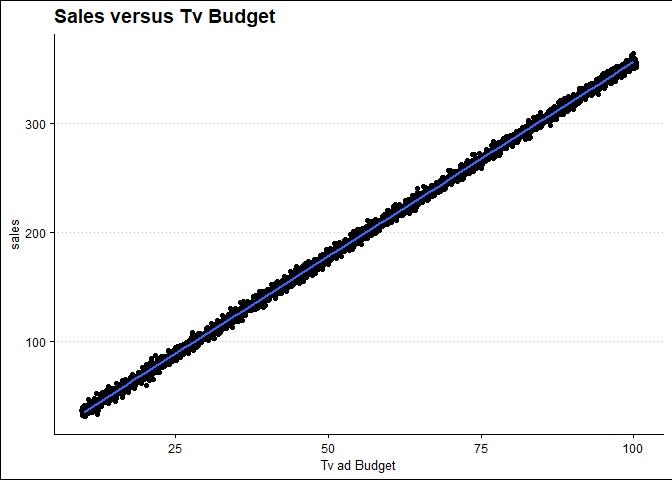
\includegraphics{cleaning_pipeline2_files/figure-latex/unnamed-chunk-4-1.pdf}

\begin{Shaded}
\begin{Highlighting}[]
\NormalTok{cleaned\_fifa\_df }\SpecialCharTok{\%\textgreater{}\%} 
  \FunctionTok{group\_by}\NormalTok{(name) }\SpecialCharTok{\%\textgreater{}\%} 
  \FunctionTok{summarise}\NormalTok{(}\AttributeTok{total\_value =} \FunctionTok{sum}\NormalTok{(value)) }\SpecialCharTok{\%\textgreater{}\%} 
  \FunctionTok{slice\_max}\NormalTok{(total\_value, }\AttributeTok{n =} \DecValTok{20}\NormalTok{) }\SpecialCharTok{\%\textgreater{}\%} 
  \FunctionTok{ggplot}\NormalTok{(}\FunctionTok{aes}\NormalTok{(}\FunctionTok{fct\_reorder}\NormalTok{(name, total\_value), total\_value))}\SpecialCharTok{+}
  \FunctionTok{geom\_col}\NormalTok{(}\AttributeTok{show.legend =}\NormalTok{ F, }\AttributeTok{fill =} \StringTok{"midnightblue"}\NormalTok{, }\AttributeTok{alpha =}\NormalTok{ .}\DecValTok{9}\NormalTok{) }\SpecialCharTok{+}
  \FunctionTok{coord\_flip}\NormalTok{()}\SpecialCharTok{+}
  \FunctionTok{theme\_minimal}\NormalTok{()}\SpecialCharTok{+}
  \FunctionTok{labs}\NormalTok{(}
    \AttributeTok{title =} \StringTok{"Top 20 Fifa players by Value"}\NormalTok{,}
    \AttributeTok{x =} \StringTok{"Player"}\NormalTok{, }
    \AttributeTok{y =} \StringTok{"Value in Euros"}\NormalTok{,}
    \AttributeTok{caption =} \StringTok{"Data Source: Data Challenge"}
\NormalTok{  )}\SpecialCharTok{+}
  \FunctionTok{theme}\NormalTok{(}\AttributeTok{plot.title =} \FunctionTok{element\_text}\NormalTok{(}\AttributeTok{hjust =}\NormalTok{ .}\DecValTok{5}\NormalTok{,}\AttributeTok{colour =} \StringTok{"midnightblue"}\NormalTok{, }\AttributeTok{size =} \DecValTok{16}\NormalTok{),}
        \AttributeTok{axis.text =} \FunctionTok{element\_text}\NormalTok{(}\AttributeTok{size =} \DecValTok{16}\NormalTok{)) }
\end{Highlighting}
\end{Shaded}

\includegraphics{cleaning_pipeline2_files/figure-latex/unnamed-chunk-5-1.pdf}

\end{document}
